%==============================================================================
%  Wattchdog - Project Report (4 pages max, excluding cover)
%  Embedded Systems Architecture - Universidade de Aveiro
%  Structure:
%     §1 Objective              - 1 page
%     §2 System Architecture    - 0.5-1 page
%     §3 Software               - 1-1.5 pages
%     §4 Hardware               - 0.5 page
%
%  EXTERNAL IMAGES (place in the same folder as this .tex):
%     - hardware.jpg     (photo of the assembled circuit)
%     - grafana.png      (Grafana dashboard screenshot)
%     - logs.png         (serial output: MQTT stream + esp_pm_dump_locks + sleep stats)
%     - FinalDiagram.pdf (circuit schematic, optional - referenced in text)
%==============================================================================
\documentclass[10pt,a4paper]{article}

\usepackage[utf8]{inputenc}
\usepackage[T1]{fontenc}
\usepackage[english]{babel}
\usepackage{lmodern}
\usepackage{microtype}
\usepackage[a4paper, top=2cm, bottom=2cm, left=2cm, right=2cm]{geometry}

\usepackage{graphicx}
\usepackage{booktabs}
\usepackage{tabularx}
\usepackage{xcolor}
\usepackage{listings}
\usepackage{amsmath}
\usepackage{siunitx}
\usepackage{enumitem}
\usepackage{tikz}
\usetikzlibrary{arrows.meta, positioning}
\usepackage{caption}
\usepackage{float}
\usepackage[hidelinks]{hyperref}

\sisetup{per-mode=symbol}
\DeclareSIUnit{\byte}{B}
\DeclareSIUnit{\inch}{in}

\captionsetup{font=small, skip=3pt}
\setlist{itemsep=1pt, topsep=2pt}

\lstset{
  basicstyle=\ttfamily\scriptsize,
  backgroundcolor=\color{gray!8},
  frame=single, rulecolor=\color{gray!50},
  breaklines=true, showstringspaces=false,
  tabsize=2, captionpos=b, numbers=none,
  literate={Ω}{$\Omega$}1 {µ}{$\mu$}1 {×}{$\times$}1
}

\newcommand{\code}[1]{\texttt{\small #1}}

\title{Wattchdog\\\large Power Fault Detector for Electrical Distribution Posts}
\author{Martim Carvalho \and Diogo Zeca}
\date{May 2026}

\begin{document}

%==============================================================================
%  COVER PAGE (excluded from page count)
%==============================================================================
\begin{titlepage}
  \centering
  \vspace*{2cm}
  {\scshape\Large Universidade de Aveiro\par}
  {\scshape DETI - Embedded Systems Architecture\par}
  \vfill
  {\Huge\bfseries Wattchdog\par}
  \vspace{0.5cm}
  {\Large Power Fault Detector for Electrical Distribution Posts\par}
  \vspace{0.4cm}
  {\itshape Embedded system based on ESP32-C6\par}
  \vfill
  \begin{tabular}{rl}
    \textbf{Authors:} & Martim Carvalho \quad \texttt{martimhcarvalho@ua.pt} \\
                      & 108749 \\[2pt]
                      & Diogo Zeca \quad \texttt{dsgps@ua.pt} \\
                      & 108212 \\
  \end{tabular}
  \vfill
  {\large May 2026\par}
\end{titlepage}

%==============================================================================
%  §1 OBJECTIVE AND CONTEXT  (~1 page)
%==============================================================================
\section{Objective and Context}

In an electrical distribution network, hundreds of posts feed consumers.
When one loses power or enters an overvoltage condition, current detection is
\emph{reactive}: the operator only learns of the fault when a customer complains.
The result is a gap of several hours between the actual fault and the start of
repair, with costs that are visible to consumers and \emph{invisible} to preventive
maintenance --- particularly \emph{brownouts}, transient overvoltages that silently
degrade downstream equipment without ever triggering an immediate complaint. Over
months, these anomalies reduce the lifespan of transformers and protection equipment;
when the final failure occurs, the operator no longer has the history needed to
reconstruct the cause, and the fault appears \emph{random}.

\textbf{Wattchdog} is a smart sensor node designed to fill this gap. Each node,
built around an \textbf{ESP32-C6} microcontroller, is installed at a post and
continuously monitors the supply, classifying the grid state into three distinct
scenarios based on the bus voltage measured \emph{in situ}:

\begin{itemize}[noitemsep]
  \item \textbf{NORMAL} --- $\SI{1.0}{\volt} \le V_{bus} \le \SI{3.9}{\volt}$.
        The grid is operating within the expected range; no action required.
  \item \textbf{BROWNOUT} --- $V_{bus} > \SI{3.9}{\volt}$. Overvoltage or overload;
        \emph{medium} urgency, requires investigation before it becomes a failure.
  \item \textbf{POWER LOSS} --- $V_{bus} < \SI{1.0}{\volt}$. Power loss or short
        circuit; \emph{critical} urgency, requires immediate intervention.
\end{itemize}

Detection occurs in \textbf{less than one second}. Each scenario transition is
signalled simultaneously through two complementary channels. \emph{Locally}, at
the post itself, the system displays voltage, current and power readings on a TFT
screen, blinks an LED at a distinct rate per state, and emits an audible tone
through a buzzer whose frequency also varies with the state. \emph{Remotely}, the
node publishes its state via MQTT over WiFi, feeding a central Grafana dashboard
where the operator monitors the health of all posts in real time.

The demonstration bench includes an adjustable potentiometer ($R_3$, Section~4)
that allows the full bus voltage range to be swept manually during testing, forcing
the system to transition between the three scenarios and exposing the local (screen,
LED, buzzer) and remote (dashboard) signalling to direct observation. This approach
allows reproducible validation --- without requiring a real electrical installation
--- that each scenario is detected within the target window of \SI{1}{\second} and
that the response across all four output channels is simultaneous.

This project is driven by four course requirements: \textbf{(i)} integrate at least
one sensor; \textbf{(ii)} include at least one actuator and/or TFT/OLED screen;
\textbf{(iii)} provide network connectivity with a justified purpose; and
\textbf{(iv)} take advantage of the microcontroller's low-power modes. The following
sections describe how each of these requirements is realised in Wattchdog, from the
overall architecture to the software and hardware layers.

%==============================================================================
%  §2 SYSTEM ARCHITECTURE  (~0.5-1 page)
%==============================================================================
\section{System Architecture}

The system splits into two subsystems (Figure~\ref{fig:pipeline}): the \emph{edge},
consisting of the embedded node installed at the post, and the monitoring
\emph{backend}, running in \emph{Docker Compose} on the operator's machine. This
separation reflects a deliberate design choice: fault detection and local signalling
\emph{do not depend on the network}, so a connectivity failure silences the
telemetry but not the physical alarm at the post.

\begin{figure}[H]
\centering
\resizebox{0.95\textwidth}{!}{%
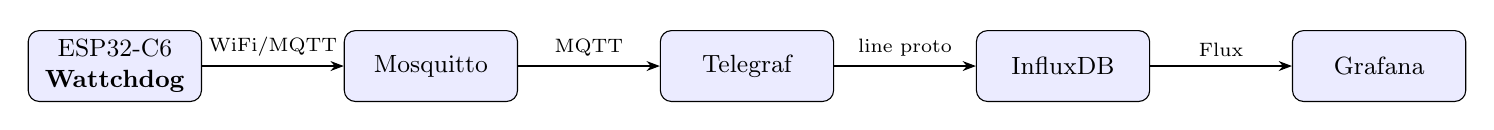
\begin{tikzpicture}[node distance=1.8cm, font=\small, >=Stealth,
  box/.style={draw, rounded corners, minimum height=0.9cm, minimum width=2.2cm, align=center, fill=blue!8}]
  \node[box] (esp) {ESP32-C6\\\textbf{Wattchdog}};
  \node[box, right=of esp] (mq) {Mosquitto};
  \node[box, right=of mq] (tg) {Telegraf};
  \node[box, right=of tg] (idb) {InfluxDB};
  \node[box, right=of idb] (gf) {Grafana};
  \draw[->] (esp) -- node[above, midway, font=\scriptsize]{WiFi/MQTT} (mq);
  \draw[->] (mq) -- node[above, midway, font=\scriptsize]{MQTT} (tg);
  \draw[->] (tg) -- node[above, midway, font=\scriptsize]{line proto} (idb);
  \draw[->] (idb) -- node[above, midway, font=\scriptsize]{Flux} (gf);
\end{tikzpicture}}
\caption{Telemetry pipeline, from the embedded node (edge) to the operator's dashboard.}
\label{fig:pipeline}
\end{figure}

At the \emph{edge}, the ESP32-C6 reads the INA219 sensor over I\textsuperscript{2}C,
classifies the state against the voltage thresholds, and simultaneously drives the
screen, LED and buzzer; it then publishes a JSON message on an MQTT topic identified
by the node's MAC address. In the \emph{backend}, the \textbf{Mosquitto} broker
routes the messages; \textbf{Telegraf} consumes them and flushes to InfluxDB every
\SI{2}{\second}; \textbf{InfluxDB} persists them as a time series; and \textbf{Grafana}
(Figure~\ref{fig:grafana}) provides dashboards for the operator, with panels for
voltage/current/power, colour-coded textual classification, and a node light sleep
indicator.

\begin{figure}[H]
\centering
\includegraphics[width=0.85\textwidth]{grafana}
\caption{Grafana dashboard showing voltage, current and power in real time, the state
panel (here in BROWNOUT) and the node light sleep indicator (\emph{AWAKE} during a
state transition).}
\label{fig:grafana}
\end{figure}

%==============================================================================
%  §3 SOFTWARE  (~1-1.5 pages)
%==============================================================================
\section{Software}

The firmware runs on \textbf{ESP-IDF} (FreeRTOS) and is organised around three
independent tasks that communicate through a shared data structure \code{g\_data}
protected by a \emph{mutex}. Each task has a single responsibility, which ensures
that none blocks another and that each can sleep whenever it has no useful work ---
the structural condition that makes \emph{light sleep} work (see below).

\paragraph{FreeRTOS tasks.} \code{task\_sensor} (\SI{1}{\hertz}) reads the INA219,
classifies the state against the thresholds described in Section~1, drives the LED
and buzzer, and updates \code{g\_data}; whenever the state changes, it notifies the
MQTT task. \code{task\_display} (\SI{2}{\hertz}) reads \code{g\_data} and refreshes
the ST7735 screen, keeping the local interface continuously updated.
\code{task\_mqtt} is \emph{event-driven}: it blocks on \code{xTaskNotifyWait} until
woken either by a state change (\emph{awake}) or by a periodic \emph{heartbeat}
($\approx$\SI{10}{\second}, \emph{sleeping}). Local signalling (LED + buzzer) is
driven by a \SI{100}{\milli\second} periodic timer (\code{esp\_timer}), allowing
blink patterns to be generated independently of the task cadence.

\paragraph{INA219 sensor and state classification.} The INA219 driver was written
from scratch on top of the ESP-IDF~v5 I\textsuperscript{2}C API. At initialisation
it configures the sensor for a \SI{16}{\volt} bus range, gain $\times 1$
($\pm$\SI{40}{\milli\volt} across the shunt), 12-bit ADCs and continuous mode. The
calibration register programs the INA219's internal multiplier so that the current
register returns values directly in \SI{10}{\micro\ampere} per LSB:
\begin{equation}
\mathrm{Cal} = \operatorname{trunc}\!\left(\frac{0.04096}{\mathrm{LSB}_I \cdot R_{shunt}}\right) = 40960,
\quad \text{with } \mathrm{LSB}_I = \SI{10}{\micro\ampere},\; R_{shunt} = \SI{0.1}{\ohm}.
\label{eq:cal}
\end{equation}
The correctness of this calibration was validated indirectly by the circuit topology
itself: since $V_{bus}$ is measured across $R_2 = \SI{1}{\kilo\ohm}$,
$I = V_{bus}/R_2$ and therefore, numerically, $I[\mathrm{mA}] \approx V_{bus}[\mathrm{V}]$.
The agreement between these two quantities, obtained by \emph{independent} ADCs
inside the INA219, confirms the measurement scale. On these calibrated readings,
state classification reduces to a threshold cascade:

\begin{lstlisting}[language=C, caption={State classification function.}]
static alert_state_t evaluate_state(float v)
{
    if (v < THRESH_POWER_LOSS) return ALERT_POWER_LOSS;  /* < 1.0 V */
    if (v > THRESH_BROWNOUT)   return ALERT_BROWNOUT;    /* > 3.9 V */
    return ALERT_NORMAL;                                 /* 1.0 .. 3.9 V */
}
\end{lstlisting}

\paragraph{Connectivity and telemetry.} WiFi operates in \emph{Station} mode with
up to five reconnection attempts; a failure is \textbf{non-fatal} --- the node
continues to operate locally, ensuring the alarm does not depend on the network.
MQTT publishing (QoS~1, on topic \code{sensors/post/<id>/metrics}, with \code{<id>}
derived from the last three bytes of the MAC) is triggered by two complementary
events: \textbf{state change} (\code{lp\_mode=0}, immediate reaction) and
\textbf{periodic heartbeat} $\approx$\SI{10}{\second} (\code{lp\_mode=1}, keep-alive
in idle state). This combination avoids flooding the broker in NORMAL state and
allows the backend to distinguish a healthy, silent node from a failed one. The
\code{lp\_mode} field is propagated from \code{task\_sensor} to \code{task\_mqtt}
via FreeRTOS notification and appears in the JSON payload:

\begin{lstlisting}[caption={JSON payload published over MQTT.}]
{"post_id":"AA:BB:CC","voltage":4.08,"current_ma":0.91,
 "power_mw":3.71,"status":"NORMAL","status_code":0,"lp_mode":1}
\end{lstlisting}

\paragraph{Low-power modes.} The adopted operating mode combines three mechanisms:
automatic \emph{light sleep} via \emph{tickless idle} (the CPU sleeps whenever all
tasks are blocked in \code{vTaskDelay}, with no code changes required),
WiFi \emph{modem sleep} (\code{WIFI\_PS\_MIN\_MODEM}, radio gated between beacons
while maintaining association), and dynamic frequency scaling (DFS) between 40 and
\SI{160}{\mega\hertz}. \emph{Deep sleep} was discarded due to unacceptable detection
latency: a fault occurring at second~1 of a \SI{30}{\second} sleep cycle would go
undetected for 29 seconds, which is unacceptable for infrastructure monitoring. The
minimum required configuration (\code{CONFIG\_PM\_ENABLE},
\code{CONFIG\_FREERTOS\_USE\_TICKLESS\_IDLE}, \code{CONFIG\_ESPTOOLPY\_FLASHSIZE\_4MB}
and the partition table) is fixed in a versioned \code{sdkconfig.defaults}, ensuring
reproducibility across machines.

The effect of \emph{light sleep} is \emph{observable} in two complementary ways. On
the dashboard (Figure~\ref{fig:grafana}), the \emph{CPU State} indicator alternates
between \emph{SLEEPING} and \emph{AWAKE}: the field \code{lp\_mode=1} is emitted
exclusively when the state is NORMAL and no transition occurred in the current cycle,
via the \SI{10}{\second} heartbeat; in BROWNOUT or POWER LOSS the heartbeat continues
to be sent but with \code{lp\_mode=0}, ensuring that the \emph{SLEEPING} indicator
faithfully reflects the node's actual idle state and not merely the absence of events.
On the serial log (Figure~\ref{fig:logs}), \code{task\_sensor} periodically dumps PM
lock statistics via \code{esp\_pm\_dump\_locks}; the table quantitatively confirms the
behaviour --- the CPU spends approximately \textbf{49\,\% of the time in light sleep
at \SI{40}{\mega\hertz}}, without losing the sub-second detection latency.

\begin{figure}[H]
\centering
\includegraphics[width=\textwidth]{logs}
\caption{Serial output of the running node: stream of published MQTT messages (top),
\code{esp\_pm\_dump\_locks} and sleep statistics table (49\,\% in light sleep,
2059 light sleep cycles counted), quantitatively proving the low-power behaviour.}
\label{fig:logs}
\end{figure}

%==============================================================================
%  §4 HARDWARE  (~0.5 page)
%==============================================================================
\section{Hardware}

The node is built around an \textbf{ESP32-C6 DevKitC-1} (RISC-V core). Measurement
is performed by the \textbf{INA219} (GY-INA219Z module), whose operating principle
relies on an internal \SI{0.1}{\ohm} shunt resistor placed in series with the load.
Because its value is small and known, the differential voltage drop across its
terminals ($V_{shunt} = I \times R_{shunt}$) is sufficient to derive the current
without breaking the circuit. The chip has two independent 12-bit ADCs: one measures
$V_{shunt}$ at \SI{10}{\micro\volt}/LSB resolution; the other measures $V_{bus}$ at
\SI{4}{\milli\volt}/LSB. With the calibration register programmed
(Equation~\ref{eq:cal}), the INA219 applies the scale factor internally and provides
current and power ($P = V_{bus} \times I$) in dedicated registers, ready to be read
over I\textsuperscript{2}C --- the microcontroller performs no floating-point
arithmetic to obtain all three quantities. The \SI{0.1}{\ohm} value results from a
trade-off: small enough not to disturb the circuit (minimal voltage drop and power
dissipation), yet large enough for $V_{shunt}$ to be accurately measurable by the
internal ADCs.

The load circuit (Figure~\ref{fig:hw}, full schematic in \code{FinalDiagram.pdf})
places $R_1 = \SI{10}{\ohm}$ (protection resistor before Vin+), the \SI{0.1}{\ohm}
shunt and $R_2 = \SI{1}{\kilo\ohm}$ in series; a potentiometer $R_3 = \SI{10}{\kilo\ohm}$
adjusts the bus voltage to the desired operating range, allowing all three scenarios
to be demonstrated during testing.

Local signalling combines three elements: an \textbf{ST7735R TFT screen}
($160 \times 80$, SPI) displaying instantaneous readings and state, a \textbf{LED}
(GP4, $+\SI{330}{\ohm}$) and a \textbf{passive buzzer} driven by PWM through the
LEDC peripheral. Unlike an active buzzer, which emits a fixed tone when powered, the
passive type \emph{allows the tone frequency to be controlled} via PWM, making it
possible to implement distinct melodies per state: BROWNOUT plays a recognisable
melody while POWER LOSS emits a descending emergency alarm. The melodies are defined
by note tables (\code{note\_t}: frequency + duration in \SI{100}{\milli\second}
ticks) stepped through by the \code{esp\_timer} periodic timer, making the alarms
immediately distinguishable by ear even in a noisy environment.
Table~\ref{tab:states} summarises the complete system response for each scenario.

\begin{table}[H]
\centering
\small
\begin{tabularx}{\linewidth}{lXXXX}
\toprule
\textbf{State} & \textbf{$V_{bus}$} & \textbf{LED} & \textbf{Buzzer} & \textbf{MQTT} \\
\midrule
NORMAL     & $1.0$--$3.9$\,V & Steady ON            & Silent               & Heartbeat 10\,s \\
BROWNOUT   & $> 3.9$\,V      & Slow blink 500\,ms   & Recognisable melody  & Immediate \\
POWER LOSS & $< 1.0$\,V      & Fast blink 100\,ms   & Emergency alarm      & Immediate \\
\bottomrule
\end{tabularx}
\caption{System response across the three operating scenarios.}
\label{tab:states}
\end{table}

\begin{figure}[H]
\centering
\begin{minipage}[c]{0.28\linewidth}
  \centering
  \includegraphics[width=\linewidth]{hardware}
\end{minipage}
\hfill
\begin{minipage}[c]{0.68\linewidth}
  \centering
  \includegraphics[width=\linewidth]{Final_Diagram.png}
\end{minipage}
\caption{(Left) Physical assembly of the Wattchdog node with the ST7735 screen
displaying INA219 readings. (Right) Full circuit schematic showing the four system
zones.}
\label{fig:hw}
\end{figure}

\end{document}
